\usetikzlibrary{arrows.meta, positioning, calc, patterns}

\definecolor{poolcolor}{HTML}{4A6FA5}
\definecolor{reservecolor}{HTML}{C9714A}
\definecolor{residualcolor}{HTML}{7C93BD}
\definecolor{lp1color}{HTML}{355B8C}
\definecolor{lp2color}{HTML}{A9B9D6}
\definecolor{arrowgray}{HTML}{888888}

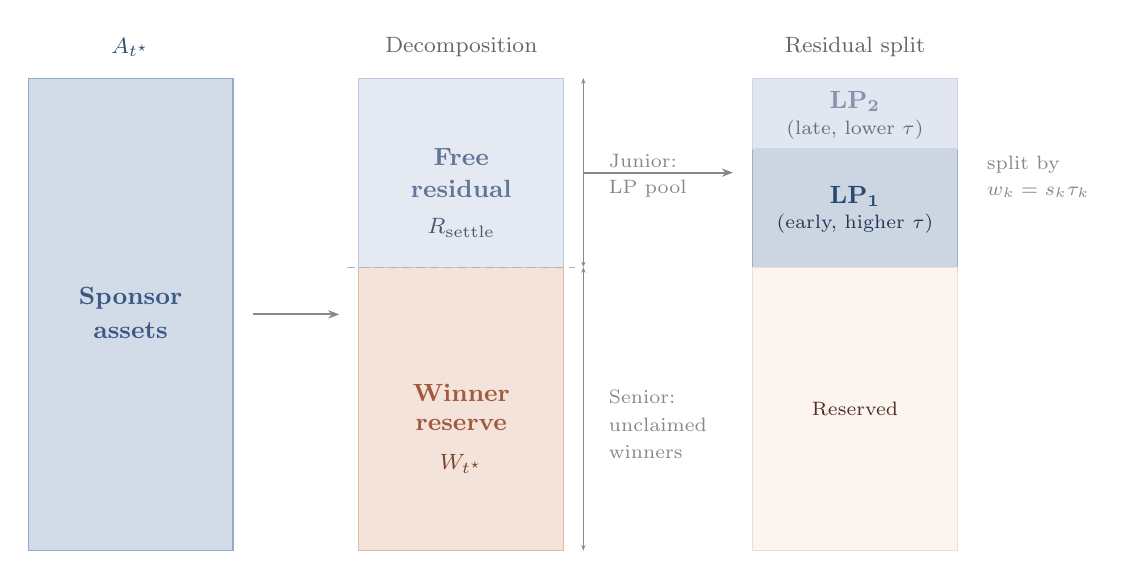
\begin{tikzpicture}[
  bar/.style={minimum width=2.6cm, draw=none, anchor=south west, inner sep=0pt},
  label/.style={font=\small, anchor=west},
]

% Column positions
\def\colA{0}       % Total pool
\def\colB{4.2}     % Decomposition
\def\colC{9.2}     % LP residual split

% Heights (proportional: total=6, reserve=3.6, residual=2.4, lp1=1.5, lp2=0.9)
\def\totalH{6}
\def\reserveH{3.6}
\def\residualH{2.4}
\def\lpOneH{1.5}
\def\lpTwoH{0.9}

% === Column A: Total pool ===
\fill[poolcolor!25] (\colA,0) rectangle ++(2.6,\totalH);
\draw[poolcolor!60, thin] (\colA,0) rectangle ++(2.6,\totalH);
\node[font=\small\bfseries, poolcolor!80!black] at (\colA+1.3, \totalH/2 + 0.2) {Sponsor};
\node[font=\small\bfseries, poolcolor!80!black] at (\colA+1.3, \totalH/2 - 0.2) {assets};
\node[font=\footnotesize, anchor=south, poolcolor!70!black] at (\colA+1.3, \totalH+0.15) {$A_{t^\star}$};

% === Column B: Reserve + Residual ===
% Reserve (bottom)
\fill[reservecolor!20] (\colB,0) rectangle ++(2.6,\reserveH);
\draw[reservecolor!50, thin] (\colB,0) rectangle ++(2.6,\reserveH);
\node[font=\small\bfseries, reservecolor!80!black] at (\colB+1.3, \reserveH/2 + 0.2) {Winner};
\node[font=\small\bfseries, reservecolor!80!black] at (\colB+1.3, \reserveH/2 - 0.2) {reserve};
\node[font=\footnotesize, reservecolor!60!black] at (\colB+1.3, \reserveH/2 - 0.7) {$W_{t^\star}$};

% Residual (top)
\fill[residualcolor!20] (\colB,\reserveH) rectangle ++(2.6,\residualH);
\draw[residualcolor!50, thin] (\colB,\reserveH) rectangle ++(2.6,\residualH);
\node[font=\small\bfseries, residualcolor!80!black] at (\colB+1.3, \reserveH + \residualH/2 + 0.2) {Free};
\node[font=\small\bfseries, residualcolor!80!black] at (\colB+1.3, \reserveH + \residualH/2 - 0.2) {residual};
\node[font=\footnotesize, residualcolor!60!black] at (\colB+1.3, \reserveH + \residualH/2 - 0.7) {$R_{\mathrm{settle}}$};

% Divider line
\draw[black!30, densely dashed, thin] (\colB-0.15,\reserveH) -- (\colB+2.75,\reserveH);

% Annotations for column B
\node[font=\footnotesize, anchor=south, black!60] at (\colB+1.3, \totalH+0.15) {Decomposition};

% Reserve annotation
\draw[{Stealth[length=2pt]}-{Stealth[length=2pt]}, arrowgray, thin]
  (\colB+2.85, 0) -- (\colB+2.85, \reserveH);
\node[font=\scriptsize, arrowgray, anchor=west, align=left] at (\colB+3.05, \reserveH/2 + 0.15) {Senior:};
\node[font=\scriptsize, arrowgray, anchor=west, align=left] at (\colB+3.05, \reserveH/2 - 0.2) {unclaimed};
\node[font=\scriptsize, arrowgray, anchor=west, align=left] at (\colB+3.05, \reserveH/2 - 0.55) {winners};

% Residual annotation
\draw[{Stealth[length=2pt]}-{Stealth[length=2pt]}, arrowgray, thin]
  (\colB+2.85, \reserveH) -- (\colB+2.85, \totalH);
\node[font=\scriptsize, arrowgray, anchor=west] at (\colB+3.05, \reserveH + \residualH/2 + 0.15) {Junior:};
\node[font=\scriptsize, arrowgray, anchor=west] at (\colB+3.05, \reserveH + \residualH/2 - 0.2) {LP pool};

% === Column C: LP split ===
% LP1 (bottom, larger share -- entered earlier, time-weighted)
\fill[lp1color!25] (\colC,\reserveH) rectangle ++(2.6,\lpOneH);
\draw[lp1color!50, thin] (\colC,\reserveH) rectangle ++(2.6,\lpOneH);
\node[font=\small\bfseries, lp1color!80!black] at (\colC+1.3, \reserveH + \lpOneH/2 + 0.15) {LP\textsubscript{1}};
\node[font=\scriptsize, lp1color!60!black] at (\colC+1.3, \reserveH + \lpOneH/2 - 0.2) {(early, higher $\tau$)};

% LP2 (top, smaller share -- entered later)
\fill[lp2color!35] (\colC,\reserveH+\lpOneH) rectangle ++(2.6,\lpTwoH);
\draw[lp2color!60, thin] (\colC,\reserveH+\lpOneH) rectangle ++(2.6,\lpTwoH);
\node[font=\small\bfseries, lp2color!80!black] at (\colC+1.3, \reserveH + \lpOneH + \lpTwoH/2 + 0.15) {LP\textsubscript{2}};
\node[font=\scriptsize, lp2color!60!black] at (\colC+1.3, \reserveH + \lpOneH + \lpTwoH/2 - 0.2) {(late, lower $\tau$)};

% Reserve block below (grayed, same as col B)
\fill[reservecolor!8] (\colC,0) rectangle ++(2.6,\reserveH);
\draw[reservecolor!25, thin] (\colC,0) rectangle ++(2.6,\reserveH);
\node[font=\scriptsize, reservecolor!40!black] at (\colC+1.3, \reserveH/2) {Reserved};

\node[font=\footnotesize, anchor=south, black!60] at (\colC+1.3, \totalH+0.15) {Residual split};

% Split formula annotation
\node[font=\scriptsize, arrowgray, anchor=west, align=left] at (\colC+2.85, \reserveH + \residualH/2 + 0.1) {split by};
\node[font=\scriptsize, arrowgray, anchor=west] at (\colC+2.85, \reserveH + \residualH/2 - 0.25) {$w_k = s_k \tau_k$};

% === Arrows between columns ===
\draw[-{Stealth[length=4pt]}, arrowgray, thick]
  (\colA+2.6+0.25, \totalH/2) -- (\colB-0.25, \totalH/2);

\draw[-{Stealth[length=4pt]}, arrowgray, thick]
  (\colB+2.6+0.25, \reserveH + \residualH/2) -- (\colC-0.25, \reserveH + \residualH/2);

\end{tikzpicture}
